\documentclass{beamer}
\setbeamercovered{transparent}
\mode<presentation>
{
  \usetheme{default}      % or try Darmstadt, Madrid, Warsaw, ...
  \usecolortheme{default} % or try albatross, beaver, crane, ...
  \usefonttheme{default}  % or try serif, structurebold, ...
  \setbeamertemplate{navigation symbols}{}
  \setbeamertemplate{caption}[numbered]
} 
\definecolor{links}{HTML}{2A1B81}
\hypersetup{colorlinks,linkcolor=,urlcolor=links}
\usepackage{tikz}
\usetikzlibrary{decorations.pathreplacing}
\usetikzlibrary{decorations.pathmorphing}
\usetikzlibrary{arrows}
\usetikzlibrary{decorations.markings}
\usetikzlibrary{decorations.pathreplacing}
\usetikzlibrary{backgrounds}
\usetikzlibrary{calc}
\usetikzlibrary{intersections}
\usetikzlibrary{decorations}
\usetikzlibrary{shapes, positioning} 
\usetikzlibrary{shadows}
\usepackage{relsize}
\tikzset{fontscale/.style = {font=\relsize{#1}}
}
\tikzstyle{line}=[draw,thick,-latex]
\setbeamerfont{block title}{size=\large}
\setbeamerfont{frametitle}{size=\Huge}
\setbeamertemplate{frametitle}[default][center]
\setbeamertemplate{footline}[frame number]
\usepackage[many]{tcolorbox}
\usepackage{empheq}
%\usepackage{3dplot} 

%\tcbset{}

%\newtcbox{\mybox}{}


\tcbset{highlight math style={colframe=red!60!black,colback=yellow!50!white,arc=4pt,boxrule=1pt,
  }}

\newtcbox{\mybox}{math upper,tcbox raise base,
  enhanced,frame hidden,boxrule=0pt,interior style={top color=green!10!white,
  bottom color=green!10!white,middle color=green!50!yellow},
  fuzzy halo=1pt with green,drop large lifted shadow}



%
% Choose how your presentation looks.
%
% For more themes, color themes and font themes, see:
% http://deic.uab.es/~iblanes/beamer_gallery/index_by_theme.html
%
\mode<presentation>
{
  \usetheme{default}      % or try Darmstadt, Madrid, Warsaw, ...
  \usecolortheme{default} % or try albatross, beaver, crane, ...
  \usefonttheme{default}  % or try serif, structurebold, ...
  \setbeamertemplate{navigation symbols}{}
  \setbeamertemplate{caption}[numbered]
} 

\usepackage[english]{babel}
\usepackage[utf8x]{inputenc}



\newcommand\pgfmathsinandcos[3]{%
  \pgfmathsetmacro#1{sin(#3)}%
  \pgfmathsetmacro#2{cos(#3)}%
}
\newcommand\LongitudePlane[3][current plane]{%
  \pgfmathsinandcos\sinEl\cosEl{#2} % elevation
  \pgfmathsinandcos\sint\cost{#3} % azimuth
  \tikzset{#1/.style={cm={\cost,\sint*\sinEl,0,\cosEl,(0,0)}}}
}

\newcommand\LatitudePlane[3][current plane]{%
  \pgfmathsinandcos\sinEl\cosEl{#2} % elevation
  \pgfmathsinandcos\sint\cost{#3} % latitude
  \pgfmathsetmacro\yshift{\cosEl*\sint}
  \tikzset{#1/.style={cm={\cost,0,0,\cost*\sinEl,(0,\yshift)}}} %
}
\newcommand\NewLatitudePlane[4][current plane]{%
  \pgfmathsinandcos\sinEl\cosEl{#3} % elevation
  \pgfmathsinandcos\sint\cost{#4} % latitude
  \pgfmathsetmacro\yshift{#2*\cosEl*\sint}
  \tikzset{#1/.style={cm={\cost,0,0,\cost*\sinEl,(0,\yshift)}}} %
}
\newcommand\DrawLongitudeCircle[2][1]{
  \LongitudePlane{\angEl}{#2}
  \tikzset{current plane/.prefix style={scale=#1}}
   % angle of "visibility"
  \pgfmathsetmacro\angVis{atan(sin(#2)*cos(\angEl)/sin(\angEl))} %
  \draw[current plane] (\angVis:1) arc (\angVis:\angVis+180:1);
  %\draw[current plane,dashed] (\angVis-180:1) arc (\angVis-180:\angVis:1);
}
\newcommand\DrawLatitudeCircle[2][1]{
  \LatitudePlane{\angEl}{#2}
  \tikzset{current plane/.prefix style={scale=#1}}
  \pgfmathsetmacro\sinVis{sin(#2)/cos(#2)*sin(\angEl)/cos(\angEl)}
  % angle of "visibility"
  \pgfmathsetmacro\angVis{asin(min(1,max(\sinVis,-1)))}
  \draw[current plane] (\angVis:1) arc (\angVis:-\angVis-180:1);
  \draw[current plane,dashed] (180-\angVis:1) arc (180-\angVis:\angVis:1);
}


\tikzset{
    MyPerspective/.style={scale=1.8,x={(-1cm,0cm)},y={(1cm,0cm)},
    z={(0cm,1.2cm)}}
        }

\title[]{Timepix3 in the AEgIS experiment}
\author{Helga Holmestad}
\institute{University of Oslo}
\date{19/9-2018}

\begin{document}

\begin{frame}
  \titlepage
\end{frame}

% Uncomment these lines for an automatically generated outline.
%\begin{frame}{Outline}
%  \tableofcontents
%\end{frame}

  \tikzstyle{line} = [draw, ultra thick,-latex]
      \tikzstyle{light} = [draw,ultra thick,yellow,-latex]
      \tikzstyle{lineP} = [draw, ultra thick]
      \tikzstyle{block} = [rectangle, draw, fill=blue, 
        text width=6.0cm, text centered, rounded corners, minimum height=1em]
      
\begin{frame}{\centering Special relativity}
  \begin{columns}
    \begin{column}{0.5\textwidth}
      \begin{itemize}
      \item{Unsolved problems at that time}
        \begin{itemize}
        \item{What is the speed of light}
        \item{Maxwells equations not consistent with relative speed of light in eter}
        \end{itemize}
      \item{Postulates}
        \begin{itemize}
        \item{Laws of physics is the same in all reference frames}
        \item{Speed of light is constant}
        \end{itemize}
      \item{Groundbreaking new ideas}
        \begin{itemize}
        \item{Space and time is not independent}
        \item{Simulationous depends upon reference frames}
        \end{itemize}
      \end{itemize}
    \end{column}
    \begin{column}{0.5\textwidth}
      \begin{center}
      \begin{tikzpicture}
        \visible<1>{
        \node at (-2,0)(man1) {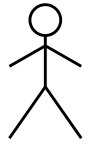
\includegraphics[width=1cm]{fig/streken.png}};  
        \node at (2,0)(man2) {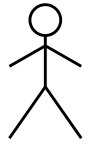
\includegraphics[width=1cm]{fig/streken.png}};  
        \path[lineP] (0,1)--(0,-1);
        \visible<1>{\path[light] ($(man1)+(4.5mm,1mm)$)--(0,1mm);}
        \visible<1>{\path[light] ($(man2)+(-4.5mm,1mm)$)--(0,1mm);}
        }
        \visible<2->{
          \node at (-1.5,0)(man1v) {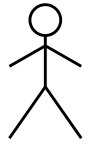
\includegraphics[width=1cm]{fig/streken.png}};  
          \node at (2.5,0)(man2v) {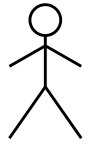
\includegraphics[width=1cm]{fig/streken.png}};  
          \path[lineP] (0.5,1)--(0.5,-1);
          \path[light] ($(man1)+(4.5mm,1mm)$)--(0,1mm);
          \path[light] ($(man2)+(-4.5mm,1mm)$)--(0,1mm);
        }
        \end{tikzpicture}
      \end{center}
    \end{column}
  \end{columns}  
\end{frame}



\begin{frame}{\centering Special relativity}
 % \begin{columns}
 %   \begin{column}{0.5\textwidth}
      By assuming the two postulates the Lorentz transformation for special relativity was derived in 1905 
      \begin{empheq}[box=\tcbhighmath]{align*}
        t'&=\beta(t-vx/c²)\\
        x'&=\beta(x-vt)\\
        y'&=y\\
        z'&=z\\
        where&:\\
        \beta&=\frac{1}{\sqrt(1-v²/c²)}
      \end{empheq}
  %    \end{column}
  \end{frame}


\begin{frame}{\centering Length contraction and time delation}
  \begin{tikzpicture}
    \draw [->, black,very thick] (0,0) -- node[below,xshift=-0.3cm]{\textbf z} (0,5);
    \draw [->, black,very thick] (0,0) --node[left,yshift=-0.3cm]{\textbf x} (5,0);
    \draw [->, gray,very thick] (0,0) --node[above]{\textbf y} (1.0,1.5);
    \node at (0,2.5){
\includegraphics[width=2cm]{fig/magic.png}};
    \draw [->, blue,very thick] (0,0) -- node[below,xshift=-0.3cm]{\textbf z'} (0,5);
    \draw [->, blue,very thick] (0,0) --node[left,yshift=-0.3cm]{\textbf x'} (5,0);
    \draw [->, blue!40,very thick] (0,0) --node[above]{\textbf y'} (1.0,1.5);

    \draw [->, blue,very thick] (0,0) -- node[below,xshift=-0.3cm]{\textbf z'} (0,5);
    \draw [->, blue,very thick] (0,0) --node[left,yshift=-0.3cm]{\textbf x'} (5,0);
    \draw [->, blue!40,very thick] (0,0) --node[above]{\textbf y'} (1.0,1.5);
    
    \node at (5,5){$\begin{aligned}v&=0.99c\\x_1&=vt\\t'&=?\\\beta&=50\end{aligned}$};
    \visible<2>{\node at (5,3){$\begin{aligned}t'_1&=\frac{t_1}{\beta}\\t_1&=\beta t'_1 \end{aligned}$};}
    %\visible<2>{\node at (5,3){$\begin{aligned}t'_1&=\frac{t_1}{\beta}\\t_1&=\beta t'_1 \end{aligned}$};}    
    \node at (5,2){The length of the carpet is 2~m, what is the length as seen by us};
    \path[lineP] (3,-0.2)--(3,0.2) node[below,yshift=-0.5cm]{$x=x_1$};
    %\visible<3>{\node at (0,0) {What is the difference between the front and the back of the magic carpent as seen from us.};}    
    %\visible<4>{\node at (5,3){$\begin{aligned} x(x'=1)-x(x'=-2)=2/\beta \end{aligned}$};}
    %\visible<5>{\node at (5,3){In other words we see that carpet as only 4~cm, instad of 2~m};}
      
    
    %\node at (0,0){
\includegraphics[width=2cm]{fig/magic.png}};
  \end{tikzpicture}
\end{frame}


\begin{frame}{Particle accelerators}
  Without time delation, the particles themself experience the time to be shorter from one end of the accelerator to the other or that we see them as taking longer time. Therefore the bunch of electrones, as you see here in CLEAR would blow up much more and not be useful in the end

\end{frame}


\begin{frame}{General relativity}

  \end{frame}
\begin{frame}{Is gravity accelration}
  \begin{columns}
    \begin{column}{0.5\textwidth}
      \begin{itemize}
      \item{In 1907 Einstein had the ``happiest thought of his life''}
      \item{There is no difference between being in an elevator in space or being in a gravitational field}
      \item{This was a continuation of the the universiality of free fall}
         
        %% \item{Two masses fall with the same accelration already seen by Galelio}
      %% \item{This lead Einstin to think: What if accelration is the same as gravity, would we know the difference}
      %% \item{Locally space can be though about as a free falling cordinate system}
      %%   \item{Free fall is where no forces is acting}
      %%   \item{We only feel gravity because the earth is massiv, so we resist the free fall}
      %% \item{Yes, you would if you where 30000 m long}
      %% \item{What if gravity was only a result of a geometry}
        \end{itemize}
         \end{column}

    \begin{column}{0.5\textwidth}
      %\begin{center}
        \begin{tikzpicture}
         % \node at (1,-4) {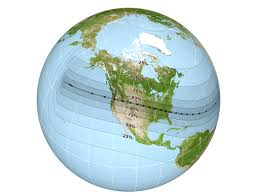
\includegraphics[width=1\textwidth]{fig/theEarth.jpg}};

        \def\x{2}
        \def\h{4}
        \def\xn{0}
        \def\hn{0}
        
        \only<1>{
          \node at (1,1.2) {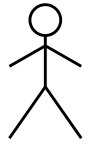
\includegraphics[width=0.25\textwidth]{fig/streken.png}};
          \path[lineP,green, line width=0.3cm] (-1,\hn-0.12cm)--(3,\hn-0.12cm);
          \node at (1,1.2) {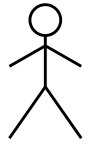
\includegraphics[width=0.25\textwidth]{fig/streken.png}};
        \path[lineP] (\hn,\xn)--(\xn,\h);
        \path[lineP] (\xn,\h)--(\x,\h);
        \path[lineP] (\x,\h)--(\x,\hn);
        \path[lineP] (\xn,\hn)--(\x,\hn);
        %\path[lineP,green] (-1,\hn)--(3,\hn);
        \node at (2.5,0.4) {
\includegraphics[width=0.07\textwidth]{fig/flower.png}};
         \node at (-0.5,0.4) {
\includegraphics[width=0.17\textwidth]{fig/grass.png}};
        
        }
        %% \def\x{4}
        %% \def\h{2}
        %% \def\xn{3}
        %% \def\hn{0}
        \only<2>{
        \draw [draw=black,fill=blue!30!black] (-1,-1) rectangle (4,5);
        \draw [draw=black,fill=white] (\xn,\hn) rectangle (\x,\h);  
        \path[lineP] (\xn,\hn)--(\xn,\h);
        \path[lineP] (\xn,\h)--(\x,\h);
        \path[lineP] (\x,\h)--(\x,\hn);
        \path[lineP] (\xn,\hn)--(\x,\hn);
        \node[star, star points=5, minimum width=0.1cm,inner sep=1.8pt,anchor=outer point 3,star point ratio=5.25, fill=yellow, draw] at (3,0.5) {};
        \node[star, star points=5, minimum width=0.1cm,inner sep=1.8pt,anchor=outer point 3,star point ratio=5.25, fill=yellow, draw] at (2.2,1.5) {};
        \node[star, star points=5, minimum width=0.1cm,inner sep=1.8pt,anchor=outer point 3,star point ratio=5.25, fill=yellow, draw] at (-0.8,1.0) {};
        \node[star, star points=5, minimum width=0.1cm,inner sep=1.8pt,anchor=outer point 3,star point ratio=5.25, fill=yellow, draw] at (0,4.2) {};
        \node[star, star points=5, minimum width=0.1cm,inner sep=1.8pt,anchor=outer point 3,star point ratio=5.25, fill=yellow, draw] at (2.5,3.7) {};
        \node at (1,1.2) {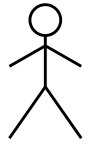
\includegraphics[width=0.25\textwidth]{fig/streken.png}};
        }
        %\draw[ultra thick] (1,2.3) circle (0.3cm);
        %\path[lineP] (0.3,1.4)--(1.0,1.8);
        %\path[lineP] (1.7,1.4)--(1.0,1.8);
        %\draw[ultra thick] (1,2.3) circle (0.3cm);
   \end{tikzpicture}
%\end{center}
    \end{column}
  \end{columns}
\end{frame}


\begin{frame}{Is gravity a geometrical effect}
  \begin{columns}
    \begin{column}{0.4\textwidth}
      \begin{itemize}
      \item{The equivalence principle is only valid locally}
      \item{Globally there is tidal forces}
      \item{Can gravity be a geometrical effect}
      \end{itemize}
    \end{column}
    \begin{column}{0.6\textwidth}
      \begin{tikzpicture}

        
        \def\x{2}
        \def\h{3}
        \def\xn{-2}
        \def\hn{1}
        
        %% \path[lineP] (\xn,\hn)--(\xn,\h);
        %% \path[lineP] (\xn,\h)--(\x,\h);
        %% \path[lineP] (\x,\h)--(\x,\hn);
        %% \path[lineP] (\xn,\hn)--(\x,\hn);

        \only<1>{
          
        \node[circle,ball color=red,shading=ball,minimum width=3cm] (ball1) at (0,-2) {};

        \node[circle,ball color=black,shading=ball,minimum width=0.3cm] (ball2) at (1,2.5) {};

        \node[circle,ball color=black,shading=ball,minimum width=0.3cm] (ball3) at (-1,2.5){};

        \path[lineP,gray,dotted] (ball1)--(ball2);
        \path[lineP,gray,dotted] (ball1)--(ball3);
        }


        \only<2,3>{
        \def\R{3 } % sphere radius
        \def\angEl{20} % elevation angle
        \def\angAz{-20} % azimuth angle
        \filldraw[shading=ball,ball color=blue] (0,0) circle (\R);
        %\filldraw[fill=white] (0,0) circle (\R);
        
        \foreach \t in {0} { \DrawLatitudeCircle[\R]{\t} }
        \foreach \t in {0,30,60,90,120,150} { \DrawLongitudeCircle[\R]{\t} }
        }
        \only<2>{
        \node[circle,ball color=black,shading=ball,minimum width=0.3cm] (ball2) at (1.5,-0.9) {};
        
        \node[circle,ball color=black,shading=ball,minimum width=0.3cm] (ball3) at (-1.5,-0.9){};
        }
        
        \only<3>{
        \node[circle,ball color=black,shading=ball,minimum width=0.3cm] (ball2) at (0.8,1.9) {};
        
        \node[circle,ball color=black,shading=ball,minimum width=0.3cm] (ball3) at (-0.8,1.9){};
        }
        
      \end{tikzpicture}
    \end{column}
  \end{columns}
\end{frame}



\begin{frame}{A geometrical model for gravity}
\begin{itemize}
\item{A manifold is a space that is curved, but locally in one point flat}
\item{The surface of a sphere is a manifold}
\item{General relativity describes space as a manifold}
\item{Locally it can be described as a free falling coordinate system, the weak equivalence principle holds}
\item{Describing space as a manifold gave the theory a  mathematical framework,  namely the mathematics of tensor analysis}
\item{}
\end{itemize}
\end{frame}
  
\begin{frame}{Einsteins field equations}
  \begin{columns}
    \begin{column}{0.5\textwidth}
      \begin{itemize}
      \item{By describing space by this manifold, and requireing that Newtons mechanics holds for low energies the Einstein field equation was derived}
      \item{Left side of the equation describes the curvature of space, metric $g_{\mu_nu}$}
      \item{The metric is the input to the geodesic equation, that gives the paths objects will move if no force is acting}
      \item{$\Lambda$ is the cosmological constant}
      \item{$T_{\mu \nu}$ is the stress-energy tensor, describes the energy in space time}
      \end{itemize}
    \end{column}
    \begin{column}{0.5\textwidth}
  
  \begin{empheq}[box=\tcbhighmath]{align*}
    R_{\mu \nu} - {1 \over 2}g_{\mu \nu}\,R + g_{\mu \nu} \Lambda = 
       {8 \pi G \over c^4} T_{\mu \nu}
       \end{empheq}
  \end{column}
  \end{columns}
\end{frame}


%% \begin{frame}{Gravity and frequency of light and your GPS}
%%   \begin{columns}
%%     \begin{column}{0.5\textwidth}
%%       \begin{itemize}
%%       \item{Given that the equivalence principle holds, what happens with light  emitted from the floor}
%%       \end{itemize}
%%     \end{column}
%%     \begin{column}{0.5\textwidth}
%%       \includegrapics{fig/solar.jpg}
%%     \end{column}
%%   \end{columns}
%% \end{frame}
  



%% \begin{frame}{Gravity and light}

%%   \begin{columns}
%%     \begin{column}{0.5\textwidth}
%%       \begin{itemize}
%%       \item{Given that the equivalence principle holds, what happens with light }
%%       \item{What happens to position of stars}
%%       \item{This can be tested, when there is a solar eclipse}
%%       \end{itemize}
%%          \end{column}
%%     \begin{column}{0.5\textwidth}
%%       \includegrapics{fig/solar.jpg}
%%     \end{column}
%%   \end{columns}
%% \end{frame}
  

    




\end{document}
%% \path[lineP] (0.3,0)--(1,1);
%% \path[lineP] (1,1)--(1.7,0);
%% \path[lineP] (1,1)--(1,2);
%% \path[lineP] (0.3,1.4)--(1.0,1.8);
%% \path[lineP] (1.7,1.4)--(1.0,1.8);
%% \draw[ultra thick] (1,2.3) circle (0.3cm);
        
        
